\documentclass[aspectratio=169]{beamer}
\usetheme{Madrid}
\usecolortheme{dolphin}
\setbeamertemplate{navigation symbols}{} % Remove nav symbols
\setbeamertemplate{itemize items}[circle]
\usepackage{graphicx}
\usepackage[utf8]{inputenc}
\usepackage{amsmath}
\usepackage{amsfonts}
\usepackage{amssymb}
\usepackage{tikz}
\usepackage{booktabs}
\usetikzlibrary{positioning, arrows.meta, shapes.geometric, calc, decorations.pathmorphing, decorations.pathreplacing, shapes, backgrounds, fit}
\usepackage[style=apa,backend=biber]{biblatex}
\addbibresource{refs.bib}

\title{\textbf{The cybernetic Cerebellum: an empirically validated categorical formalization}}
\author{Luis Nicolas Luarte Rodriguez}
\institute{CICS}
\date{\today}

\begin{document}
	
	\begin{frame}
		\maketitle
	\end{frame}
	
	\begin{frame}{The main idea}
		\large{\textit{The Cerebellum is the cybernetic core of human behavior across modalities}}
		\begin{columns}
			
			\begin{column}{0.4\textwidth}
				\begin{block}{Cybernetics}
					A mapping between states or contexts to actions that \textbf{minimizes error} and \textbf{uncertainty}.
					
					$$State_{Hungry} \rightarrow Eat$$
					$$State_{Danger} \rightarrow Run$$
				\end{block}
			\end{column}
			
			\begin{column}{0.5\textwidth}
				\begin{block}{Across-modalities}
					The process is performed in a non-representational space. Thus, it works regardless of the nature of the problem being motor, economic, or otherwise.
					
					\centering
					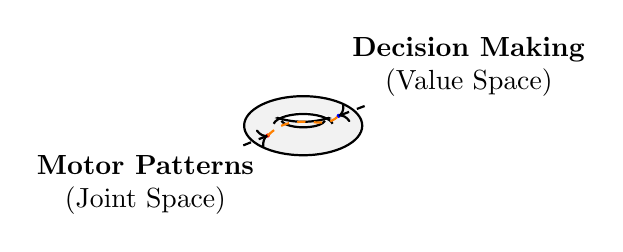
\begin{tikzpicture}[scale=0.25]
						% Draw Torus
						\draw[thick, fill=gray!10] (0,0) ellipse (3cm and 1.5cm);
						\begin{scope}
							\clip (0,-1.8) ellipse (3cm and 2.5cm);
							\draw[thick, fill=white] (0,2.2) ellipse (3cm and 2cm);
						\end{scope}
						\draw[thick] (-1.5,0.1) arc (170:10:1.52cm and 0.6cm);
						\draw[thick] (-1.1,0.25) arc (-170:-10:1.12cm and 0.4cm);
						
						% Points
						\coordinate (A) at (-1.8, -0.5);
						\coordinate (B) at (1.8, 0.5);
						
						\fill[red] (A) circle (3pt);
						\fill[blue] (B) circle (3pt);
						
						% Labels and Lines
						\node[align=center, below left] at (-2, -1) (L1) {\textbf{Motor Patterns}\\(Joint Space)};
						\draw[->, thick, dashed] (L1) -- (A);
						
						\node[align=center, above right] at (2, 1) (L2) {\textbf{Decision Making}\\(Value Space)};
						\draw[->, thick, dashed] (L2) -- (B);
						
						% Connection on Manifold
						\draw[thick, orange, dashed] (A) to[out=45, in=180] (0,0.2) to[out=0, in=225] (B);
						\node[above, black] at (0,0.2) {};
						
					\end{tikzpicture}
					
				\end{block}
			\end{column}
		\end{columns}
		
	\end{frame}
	
	\begin{frame}{Motivation: intuition for universality}
		\textbf{Intuition}: learning across modalities requires two fundamental operations:
		\begin{itemize}
			\item Context embedding: to represent state, action, value $(s, a, v)$ in a linearly separable way.
			\item Error correction: signal to modify the mapping from Embedding $\rightarrow$ Action
		\end{itemize}
		
		\begin{block}{The Marr-Albus insight \parencite{marrTheoryCerebellarCortex1969}}
			\begin{itemize}
				\item Mossy Fiber $\rightarrow$ Granule Cell (1:1)
				\item Each claw samples one input dimension from MF
				\item Granule Cells have 3-5 claws
				\item MF:GC is 1:100, (50 billion GC)
			\end{itemize}
			\[ E(L) \cong \coprod_{i} \binom{L}{R} \]
		\end{block}
		
	\end{frame}
	
	\begin{frame}{Context embedding}
		\centering
		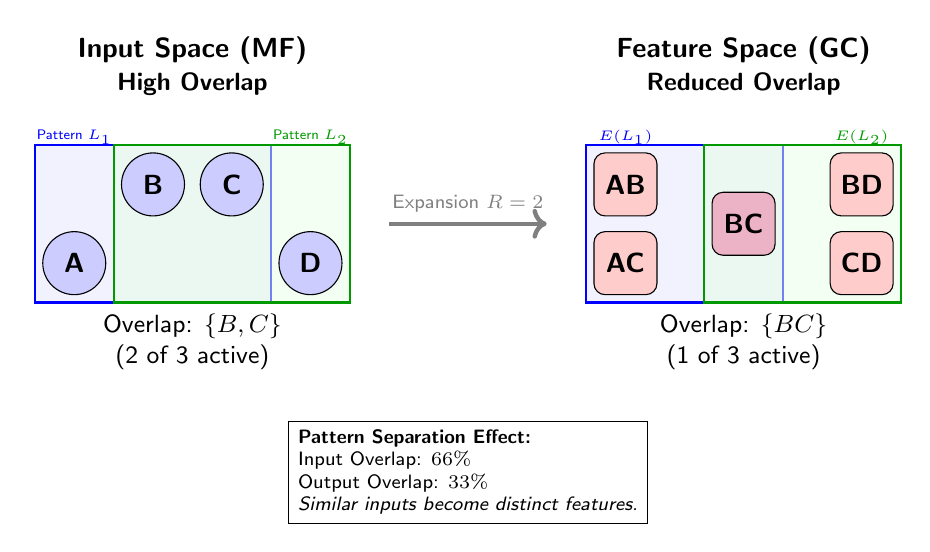
\begin{tikzpicture}[
			scale=1.0, transform shape,
			fiber/.style={circle, draw, fill=blue!20, minimum size=0.8cm, font=\sffamily\bfseries},
			granule/.style={rectangle, draw, fill=red!20, rounded corners, minimum size=0.8cm, font=\sffamily\bfseries},
			label text/.style={font=\sffamily\bfseries, align=center}
			]
			
			% --- LEFT PANEL: Input Space (Mossy Fibers) ---
			\node[label text] at (1.5, 4.5) {Input Space (MF)\\\small High Overlap};
			
			% Fibers A, B, C, D
			\node[fiber] (A) at (0, 2) {A};
			\node[fiber] (B) at (1, 3) {B};
			\node[fiber] (C) at (2, 3) {C};
			\node[fiber] (D) at (3, 2) {D};
			
			% Sets L1 and L2
			\begin{scope}[on background layer]
				\draw[blue, thick, fill=blue!10, fill opacity=0.5] (-0.5, 1.5) rectangle (2.5, 3.5);
				\node[blue, font=\sffamily\tiny] at (0, 3.6) {Pattern $L_1$};
				
				\draw[green!60!black, thick, fill=green!10, fill opacity=0.5] (0.5, 1.5) rectangle (3.5, 3.5);
				\node[green!60!black, font=\sffamily\tiny] at (3, 3.6) {Pattern $L_2$};
			\end{scope}
			
			% Highlight Overlap (B, C)
			\node[font=\sffamily\small, align=center] at (1.5, 1) {Overlap: $\{B, C\}$\\(2 of 3 active)};
			
			
			% --- ARROW: The Embedding E ---
			\draw[->, ultra thick, gray] (4, 2.5) -- (6, 2.5) node[midway, above, font=\sffamily\scriptsize] {Expansion $R=2$};
			
			
			% --- RIGHT PANEL: Feature Space (Granule Cells) ---
			\node[label text] at (8.5, 4.5) {Feature Space (GC)\\\small Reduced Overlap};
			
			% Granule Cells (Combinations)
			% From L1: {AB, AC, BC}
			% Aligning Y-coordinates to match Input Space (centered at 2.5)
			\node[granule] (AB) at (7, 3) {AB};
			\node[granule] (AC) at (7, 2) {AC};
			\node[granule, fill=purple!30] (BC) at (8.5, 2.5) {BC}; % Shared
			
			% From L2: {BC, BD, CD}
			\node[granule] (BD) at (10, 3) {BD};
			\node[granule] (CD) at (10, 2) {CD};
			
			% Sets E(L1) and E(L2)
			% Adjusting rectangles to (1.5, 3.5) range to align with input
			\begin{scope}[on background layer]
				% E(L1) boundary
				\draw[blue, thick, fill=blue!10, fill opacity=0.5] (6.5, 1.5) rectangle (9, 3.5);
				\node[blue, font=\sffamily\tiny] at (7, 3.6) {$E(L_1)$};
				
				% E(L2) boundary
				\draw[green!60!black, thick, fill=green!10, fill opacity=0.5] (8, 1.5) rectangle (10.5, 3.5);
				\node[green!60!black, font=\sffamily\tiny] at (10, 3.6) {$E(L_2)$};
			\end{scope}
			
			% Highlight Overlap
			\node[font=\sffamily\small, align=center] at (8.5, 1) {Overlap: $\{BC\}$\\(1 of 3 active)};
			
			% --- Comparison Text ---
			\node[draw, align=left, font=\sffamily\scriptsize, anchor=north] at (5, 0) {
				\textbf{Pattern Separation Effect:}\\
				Input Overlap: $66\%$\\
				Output Overlap: $33\%$\\
				\textit{Similar inputs become distinct features.}
			};
			
		\end{tikzpicture}
	\end{frame}
	
	\begin{frame}{Error correction}
		\centering
		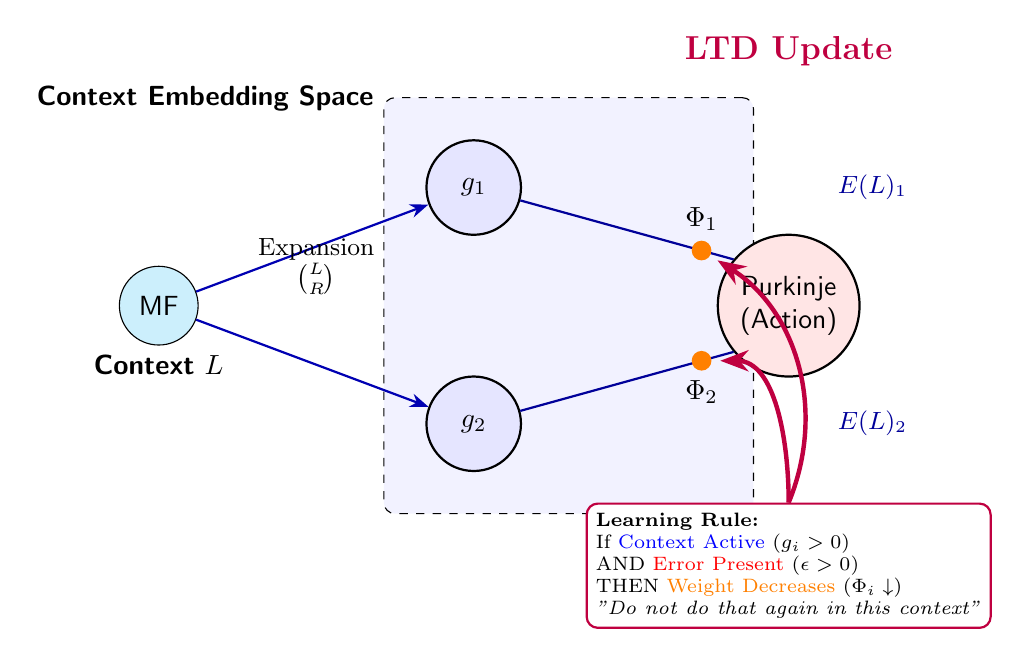
\begin{tikzpicture}[
			scale=1.0, transform shape,
			font=\sffamily,
			node distance=2cm and 3cm, % Increased spacing for clarity
			% Styles
			neuron/.style={circle, draw, thick, minimum size=1.2cm, align=center, fill=white},
			input/.style={circle, draw, fill=cyan!20, minimum size=1cm},
			synapse/.style={circle, fill=orange, minimum size=0.25cm, inner sep=0pt},
			signal/.style={->, >=Stealth, thick, draw=blue!70!black},
			error_signal/.style={->, >=Stealth, very thick, draw=red!80!black, dashed},
			ltd_action/.style={->, >=Stealth, ultra thick, draw=purple, shorten >=3pt},
			box/.style={draw, dashed, rounded corners, inner sep=15pt, fill=blue!5}
			]
			
			% --- 1. Context & Embedding ---
			\node[input, label=below:\textbf{Context $L$}] (MF) {MF};
			
			% Expansion Layer (Granule Cells) - Spaced out vertically
			\node[neuron, fill=blue!10] (GC1) at (4, 1.5) {$g_1$};
			\node[neuron, fill=blue!10] (GC2) at (4, -1.5) {$g_2$};
			
			% Connections MF -> GC
			\draw[signal] (MF) -- (GC1);
			\draw[signal] (MF) -- (GC2);
			
			% Expansion Label (Centered)
			\node[font=\small, align=center] at (2, 0.5) {Expansion\\$\binom{L}{R}$};
			
			% --- 2. Action Selection (Purkinje) ---
			% Placed further right
			\node[neuron, fill=red!10, minimum size=1.8cm] (PC) at (8, 0) {Purkinje\\(Action)};
			
			% Parallel Fibers & Synapses
			% Draw lines from GC to PC, with synapses at the junction
			\draw[thick, blue!60!black] (GC1) -- (PC.140) coordinate[pos=0.85] (S1_pos);
			\draw[thick, blue!60!black] (GC2) -- (PC.220) coordinate[pos=0.85] (S2_pos);
			
			% Synapse Nodes
			\node[synapse, label=above:$\Phi_1$] (S1) at (S1_pos) {};
			\node[synapse, label=below:$\Phi_2$] (S2) at (S2_pos) {};
			
			% Labels for Embedding
			\node[right, blue!60!black, font=\small] at (8.5, 1.5) {$E(L)_1$};
			\node[right, blue!60!black, font=\small] at (8.5, -1.5) {$E(L)_2$};
			
			% --- 3. The Cybernetic Mechanism (LTD) ---
			
			% Learning Rule Box (Simplified and moved down)
			\node[align=left, font=\scriptsize, draw=purple, thick, fill=white, rounded corners, anchor=north] (Rule) at (8, -2.5) {
				\textbf{Learning Rule:}\\
				If \textcolor{blue}{Context Active} ($g_i > 0$)\\
				AND \textcolor{red}{Error Present} ($\epsilon > 0$)\\
				THEN \textcolor{orange}{Weight Decreases} ($\Phi_i \downarrow$)\\
				\textit{"Do not do that again in this context"}
			};
			
			% LTD Arrows (From Rule Box to Synapses)
			% Representing the "Error" effect
			\draw[ltd_action, out=90, in=0] (Rule.north) to (S2);
			\draw[ltd_action, out=90, in=0] (Rule.north) to [bend right=40] (S1);
			
			% Label for the whole process
			\node[font=\bfseries\large, purple, above=of PC] {LTD Update};
			
			
			% --- Background grouping ---
			\begin{scope}[on background layer]
				\node[box, fit=(GC1) (GC2) (S1) (S2), label=above left:\textbf{Context Embedding Space}] {};
			\end{scope}
			
		\end{tikzpicture}
	\end{frame}
	
	\begin{frame}{The research question}
		\large{Is the biological circuit of the Cerebellum an implementation of the 'Bellman Equation' (the fundamental formula for learning from mistakes and to optimize any behavior), whether motor or cognitive, simply by minimizing prediction error?}
	\end{frame}
	
	\begin{frame}{The gap}
		\begin{itemize}
			\item \textbf{Micro}: We have very specific models for sparse connectivity decorrelation \parencite{cayco-gajicSparseSynapticConnectivity2017}, and for synaptic plasticity rules to behavioral timing \parencite{suvrathanTimingRulesSynaptic2016}, among many others. However, they often fail to explain what high-level function is being optimized
			\item \textbf{Macro}: we have cerebellum-cortical model of action encoding \parencite{herzfeldEncodingActionPurkinje2015}, and reward prediction error implementation \parencite{heffleyClassicalConditioningDrives2019}. However, they are not derived from the underlying circuit topology or are 'partial' models
			\item \textbf{Consequence}: scale + identity problems
		\end{itemize}
	\end{frame}
	
	\begin{frame}{Contribution}
		\begin{itemize}
			\item Generate a meso-level generative category that determines global structure from local function
		\end{itemize}
		
	\end{frame}
	
	\begin{frame} {Paper I the unified model}
		The Objective is to generate a category for the Cerebellum, which is composed of:
		\begin{itemize}
			\item \textbf{Objects}: represent the functional information states, such as the set of Mossy Fibers, the set of Granule Cells, and the set of Purkinje Cell output rates
			\item \textbf{Morphisms}: map the state of one population to another
			\item \textbf{Optics (Bellman)}: provide explicit rules to morphisms
		\end{itemize}
		After the category is generated, running the optics through it yields hypotheses necessary for preserving local and global structure. Similar to how game theory finds 'balances' in games.
	\end{frame}
	
	\begin{frame}
		After theoretical validation, we perform the empirical validation:
		\begin{itemize}
			\item \textbf{Entity linking}: for morphism $A \rightarrow B$ translate objects into canonical identifiers (e.g. MeSH terms) using BERN2
			\item \textbf{Proposition generation}: transform $A \xrightarrow{R} B$ into a testeable sentence using (search in PUBMED)
			\item \textbf{Semantic matching}: (a) get a similarity vector of sentences, (b) derive directionality using zero-shot classification $A \xrightarrow{inhibits} B$ or $A \xrightarrow{excites} B$
			\item \textbf{Network Structure learning}: based on results generate a proposal $\mathcal{C'}$ that improves category quality (optics) and empirical support
			\item \textbf{Outcome}: between task similarity
		\end{itemize}
		
		This yields something similar to a systematic review, with the added benefit of an explicit model and hypothesis proposal.
	\end{frame}
	
	\begin{frame}{Paper II neural isomorphism}
		Show correlation-level validation. Is the map real?
		\begin{itemize}
			\item \textbf{Experiment}: fMRI + EEG recordings during an economic decision task (two-armed bandit) and motor learning task (visomotor adaptation)
			\item \textbf{Analysis}: representational similarity analysis. For both tasks, take comparable task states (low/high error, low/high uncertainty) and correlate them with neural signatures (informed by category morphisms) (BOLD signal, spectral-power). Do the subject partitions at the neural level show similar task states across tasks?
		\end{itemize}
	\end{frame}
	
	\begin{frame}{Paper III in-silico cerebellum}
		\begin{itemize}
			\item \textbf{Objective}: develop a computational agent model, based on paper I
			\item \textbf{Goodness of fit}: compare the model predictive power against staple learning models, fitting data from paper II
			\item \textbf{Causal hypothesis}: use the model to generate a prediction of what happens when specific pathways are blocked (the model is a mirror of $\mathcal{C}$)
		\end{itemize}
	\end{frame}
	
	\begin{frame}{Paper IV causal validation}
		\begin{itemize}
			\item \textbf{Experiment}: same task as paper II. Apply transcranial magnetic stimulation to the cerebellar cortex, knowing the object-morphism previously validated
			\item \textbf{Hypothesis}: derived from paper III
			\item \textbf{Outcome}: causal evidence for cerebellum universal function and the category formalization
		\end{itemize}
	\end{frame}
	
	\begin{frame}{References}
		\printbibliography
	\end{frame}
	
\end{document}